% Template for Cogsci submission with R Markdown

% Stuff changed from original Markdown PLOS Template
\documentclass[10pt, letterpaper]{article}

\usepackage{cogsci}
\usepackage{pslatex}
\usepackage{float}

% amsmath package, useful for mathematical formulas
\usepackage{amsmath}

% amssymb package, useful for mathematical symbols
\usepackage{amssymb}

% hyperref package, useful for hyperlinks
\usepackage{hyperref}

% graphicx package, useful for including eps and pdf graphics
% include graphics with the command \includegraphics
\usepackage{graphicx}

% Sweave(-like)
\usepackage{fancyvrb}
\DefineVerbatimEnvironment{Sinput}{Verbatim}{fontshape=sl}
\DefineVerbatimEnvironment{Soutput}{Verbatim}{}
\DefineVerbatimEnvironment{Scode}{Verbatim}{fontshape=sl}
\newenvironment{Schunk}{}{}
\DefineVerbatimEnvironment{Code}{Verbatim}{}
\DefineVerbatimEnvironment{CodeInput}{Verbatim}{fontshape=sl}
\DefineVerbatimEnvironment{CodeOutput}{Verbatim}{}
\newenvironment{CodeChunk}{}{}

% cite package, to clean up citations in the main text. Do not remove.
\usepackage{cite}

\usepackage{color}

% Use doublespacing - comment out for single spacing
%\usepackage{setspace}
%\doublespacing


% % Text layout
% \topmargin 0.0cm
% \oddsidemargin 0.5cm
% \evensidemargin 0.5cm
% \textwidth 16cm
% \textheight 21cm

\title{The importance of alternatives in scalar implicature}


\author{{\large \bf Benjamin Peloquin} \\ \texttt{bpeloqui@stanford.edu} \\ Department of Psychology \\ Stanford University \And {\large \bf Michael C. Frank} \\ \texttt{mcfrank@stanford.edu} \\ Department of Psychology \\ Stanford University}

\begin{document}

\maketitle

\begin{abstract}
Succesful communication regularly requires listeners to make pragmatic
inferences - enrichments beyond the literal meaning of a speaker's
utterance. For example, listeners routinely enrich the meaning of
``some'' to ``some, but not all'' when interpreting a sentence such as
``Bob ate some of the cookies.'' A Gricean account of this phenomena
assumes the presence of \emph{salient alternatives} with varying degrees
of informativity. ``Some,'' in the example above, is enriched to ``some,
but not all'' in the presence of the stronger alternative ``all.''
Empirical evidence for the presence of such alternatives and accounts of
their effect on implicature has been limited. Our current work explores
the role different scale representations may play in scalar implicature
using empirical measures of literal semantics and a Bayesian model of
implicature generation. Comparisons with human judgments indicate that
pragmatic inference may rely on fairly complete alternative sets rather
than the typical entialment only scales assumed in most research to
date.

\textbf{Keywords:}
pragmatics; scalar implicature; bayesian modeling
\end{abstract}

\section{Introduction}\label{introduction}

Humpty Dumpty Quote\ldots{}

Successful communication regularly requires listeners to make inferences
that go beyond the literal semantic content of a speaker's utterance.
``Scalar implicature'' is a hallmark of such pragmatic enrichment. For
example, listeners routinely enrich the meaning of the scalar item
``some'' to ``some, but not all'' in sentences like ``Bob ate some of
the cookies'' (van Tiel, 2014; other\ldots{}). A Gricean account of this
phenomena assumes listeners reason about the intended meaning of a
speaker while incorporating knowledge about a) alternative scalar items
a speaker could have used (such as ``all'') and b) the relative
informativity of using such alternatives (Grice, 1975). Under the
Gricean account, a listener will infer that the speaker must have
intended that Bob did not eat ``all'' the cookies because it would have
been \emph{underinformative} for the speaker to use ``some'' when
``all'' could have been used.

The presence of ``salient" alternatives is critical to the standard
Gricean account of scalar implicature (Grice, 1975). Recent experimental
evidence appears to support this. Using a gumball paradigm, Degen \&
Tanenhaus (2014) demonstrated that the scalar item \emph{some} was
judged less appropriate (natural) for small sets of items when exact
numbers were seen as viable alternatives. This finding points to the
impact a particular alternative set can have on judgments regarding
scalar appropriateness. Using a fundamentally different approach, Franke
(2014) formalized the Gricean account of implicature using a Bayesian
model, modeling graded typicality judgments and scalar implicature.
Results supported `none', `one' and `all' as the most serious (salient)
alternatives to ``some.''

Taken together, each of the previous studies signal the importance of
scale representation (set of available alternatives) in scalar
implicature. However, like many recent investigations which have focused
only on a small subset of scalar items, both Degen \& Tanenhaus (2014)
and Franke (2014) focus exclusively on the scalar family ``some/all.''
This lack ``Scalar Diversity'' (van Tiel, 2014) makes generalization
across different scalar families problematic. van Tiel (2014), found
substantial variation in the rate of upper-bounded construals aross more
than 40 different scalar pairs. This finding suggests that implicature
may differ widely between different scales. We adopt a ``Scalar
Diversity'' approach in our experimental design in order to extend our
investigation beyond ``some/all'' scalar items. In the following set of
studies we examine implicature for ``some/all'' and five additional
scalar families from a range of grammatical classes (see Figure 5 for a
complete set of scalar items used). The set of scalar items for this
study were chosen from among the 40 used in van Tiel (2014).

Consider a scalar item other than ``some'' - in the context of the word
``good'', the idea of set of lexical alternatives seems intuitive
(``bad'', ``excellent'', etc.). But measuring the extent to which these
alternatives are salient is not so clear. Nor is how to measure their
impact on pragmatic interpretations of the scalar item ``good.'' In an
experimental setting, querying a participant about the saliency of a
particular alternative is problematic because the alternative must be
made salient during the query. In the spirit of Franke (2014) and Degen
\& Tanenhaus (2014), we pair a computational model of implicature with
empirical measurements of linguistic material. This combination allows
us to simulate the effect of various scale representations on
implicature. In particular, we adopt a Bayesian model of implicature and
a food-review paradigm to empirically quantify literal semantics and
pragmatic judgments for our scalar stimuli.

Bayesian models of pragmatic enrichment have accurately predicted human
judgments in ad-hoc (Frank \& Goodman, 2012) and embedded (Stulhmuller
\& Goodman, 2014) implicature settings. Our current model follows both
these studies and is based on Rational Speech-act theory (RSA). RSA
frames language understanding as a special case of social cognition
(Frank \& Goodman, 2012; Stulhmuller \& Goodman, 2014), in which
listeners and speakers reason about one-another. In this framework, a
listener uses Bayesian inference to interpret the intended meaning \(m\)
of a speaker who has made an utterance \(u\). We will make the model
specifications explicit later in the paper.

In the following study we investigate the role of scale representation
on scalar implicature. To do so we combine a computational framework
with empirical measurements to simulate the type of scale
representations that might be available to a listener. In the following
sections we outline the specifics of the model and the particular
components for which we need to to make empirical measurements. We then
outline a series of experiments meant to a) quantify literal semantics
for otherwise ambiguous scalar items, b) measure pragmatic judgments and
c) generate a set of plausible alternatives for our set of scalar pairs
taken from van Tiel (2014). In particular, we adopt a food review
paradigm throughout our empirical data gathering, quantifying linguistic
meaning (both literal semantics and pragmatic judgments) as
distributions over star ratings. Finally, we simulate the impact of
three different scale representations, ``entailment'', ``mid'' and
``symmetric'' on implicature generation, comparing model predictions
with pragmatic judgments captured empirically. Results indicate that
humans may employ more ``fully specified'' scale representations,
relying on the presence of multiple alternatives during pragmatic
enrichment.

\begin{center}\rule{0.5\linewidth}{\linethickness}\end{center}

\section{Modeling implicature: Rational Speech-act
theory}\label{modeling-implicature-rational-speech-act-theory}

We adopt a Bayesian model of scalar implicature known as Rational
Speech-act theory (RSA). In particular, RSA frames language
understanding as a special case of social cognition (Frank \& Goodman,
2012; Stuhmuller \& Goodman, 2014) in which listener and speaker agents
reason about one another. We focus on the problem of a listener
inferring the meaning of a speaker's utterance. Let \(u\) be an observed
utterance made by our speaker with an intended meaning \(m\). We assume
that the listener has access to a space of possible meanings \(M\) and
some model relating meanings \(m \in M\) to \(u\).

Upon hearing an utterance \(u\) the Listener agent evaluates all
candidate word meanings, computing their posterior probabilities
\(p_{L1}(m | u)\). This quantity is proportional to the product of the
prior probability \(p(m)\) of a particular meaning and the likelihood
\(p(u | m)\).

\[p_{L1}(m | u) = \frac{p(u | m)p(m)}{p(u)}\]
\[= \frac{p(u | m)p(m)}{\sum_{m \in M}p(u | m)}\]

The \textbf{prior} \(\mathbf{p(m)}\) represents the listener's
expectations about plausible meanings (star ratings), \emph{independent}
of the utterance \(u\). To avoid biasing the data we assume priors over
meanings are uniform, however future investigations may want to
experiment with different priors, either by inferring them or using
empirical measures

\(\mathbf{p(u | m)}\) quantifies the \textbf{likelihood} that a speaker
would make a particular utterance \(u\) given an intended meaning \(m\).
Our model assumes that speakers choose words to maximize the utility of
an utterance in context. Utility is operationalized as the informativity
of a particular utterance (surprisal) minus a cost. In particular, the
speaker chooses an utterance in order to maximize the utility of a
listener who interprets her utterance literally \(p_{L0}(m|u)\). \(L_0\)
denotes a literal listener interpretation of meaning \(m\) given
utterance \(u\).
\[p(u | m) = \frac{e^{-\alpha(-log(p_{L0}(m|u)) - cost(u))}}{\sum_{m \in M}e^{-\alpha(-log(p_{L0}(m|u)) - cost(u))}}\]

The \textbf{posterior} \(\mathbf{p_{L1}(m | u)}\) quantifies a
listener's degree of belief that a speaker intended a meaning \(m\)
given an utterance \(u\). The subscript \(L_1\) denotes a pragmatic
listener interpretation of meaning \(m\) given utterance \(u\).

\subsection{Simluating implicature: Measuring literal semantics and
pragmatic
judgments}\label{simluating-implicature-measuring-literal-semantics-and-pragmatic-judgments}

In order to simulate the role of scale representation on implicature we
pair a computational framework with empirical data. In particular we use
experimental tools to populate three components of the model. First, to
measure otherwise ambiguous literal semantics \(\mathbf{p_{L0}(m|u)}\)
(our ``Scalar Diversity''" approach). Second, to generate a set of
plausible alternatives to the original scalar pairs taken from van Tiel
(2014). Lastly, to obtain human pragmatic judgments for model comparison
\(\mathbf{p_{L1}(m|u)}\).

Starting with the first component, consider the scalar items ``some''
and ``all.'' Both are convenient for modeling in a computational
framework like the one we've proposed above. Their literal semantics
\(\mathbf{p_{L0}}\) are easily quantified over sets.

\[\text{\text it{some of the A's are B's.}}\]
\[[[some]] = \{<A, B> : |A \cap B| \geq 1 \}\]

\[\text{\text it{all of the A's are B's.}}\]
\[[[all]] = \{<A, B> : \frac{|A \cap B|}{|A|} == 1 \}\]

The same cannot be said for items such as ``good / excellent'',
``memorable / unforgettable'' or ``liked / loved.''

In the following set of studies we adopt a food-review paradigm to
measure literal semantics and pragmatic judgments empirically. In order
to capture graded typicality judgments as in Degen \& Tanenhaus (2014)
we use a compatibility measure dependent variable, pairing scalar items
with star-ratings in our literal listener task (Experiments 1a, 3a and
4). Data from these experiments is used to approximate the literal
listener semantics for a given scalar item \(u\) as a distribution over
star-ratings \(m \in \text{\{1 - 5 stars\}}\). Similarly, pragmatic
judgment data from Experiments 1b and 3b serve as our primary points of
comparison with model predictions \(\mathbf{p_{L1}(m|u)}\), again
quantifying judgments as distributions over star-ratings. In the
following section we take the reader through our experiments.

\begin{CodeChunk}
\begin{figure*}[t]

{\centering 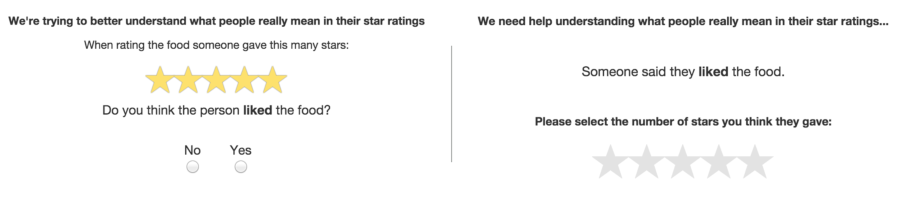
\includegraphics{figs/stimuli_exp1-1} 

}

\caption[The left panel shows a trial from Experiment 1a with the target scalar `liked']{The left panel shows a trial from Experiment 1a with the target scalar `liked'. Participants responses to the binary dependent variable are used to quantify literal semantics. The right panel shows a trial from Experiment 1b with the target scalar `liked'. Participants were asked to generate the star rating they think the speaker likely intended, given the target scalar (in this case 'liked').}\label{fig:stimuli_exp1}
\end{figure*}
\end{CodeChunk}

\section{Experiment 1a,b: Entailment
scales}\label{experiment-1ab-entailment-scales}

Experiment 1a and 1b were conducted to approximate literal listener
semantic distributions \(p_{L0}(m|u)\) (Experiment 1a) and pragmatic
judgments \(p_{L1}(m|u)\) (Experiment 1b) for five pairs of scalar items
taken from van Tiel (2014) (see figure 5 for stimuli). Each pair
consists of a ``weaker'' scalar term (e.g. ``some'') and a stronger
scalar term (e.g. ``all''). We are calling these ``entailment scales'',
because they encode the assumption that a listener need only have a the
stronger alternative present to generate an enriched interpretation of
the weaker term. The grey colored items in Table 1 denote the original
``entailment'' items used in Experiments 1a,b.

\subsection{Methods}\label{methods}

\subsubsection{Participants}\label{participants}

Participants for both tasks were recruited on Amazon Mechanical Turk and
paid \$0.20 for their participation. Thirty participants were recruited
for Experiment 1a. Data for two participants was thrown out during
analysis because they were not native English speakers, leaving a total
sample of 28 participants. Fifty participants were recruited for
Experiment 1b. Data for 7 participants was thrown out after participants
either failed to pass two training trials or were not native English
speakers, leaving a total sample of 43 participants.

\subsubsection{Design and procedure}\label{design-and-procedure}

The left panel of Figure 1 shows a screen shot of a trial from
Experiment 1a. Participants were presented with a target scalar item and
a star-rating (between 1-5 stars) and asked to judge the compatibility
of the scalar item and star-rating. Compatibility was assessed through a
binary ``yes/no'' response to a question of the form ``Do you think that
the person thought the food was \_\_\_\_?" where a target scalar was
presented in the ``\_\_\_\_." Each participant was presented all scalar
item and star-rating combinations with randomization.

The right panel of Figure 1 shows a screen shot of a trial from
Experiment 1b. On each trial, participants were presented with a
one-sentence prompt containing a target scalar item such as ``Someone
said they thought the food was \_\_\_\_\_.'' Participants were then
asked to generate a star-rating according to what they thought the
reviewer likely gave. Each participant was presented all scalar items
with randomization.

\subsection{Results and Discussion}\label{results-and-discussion}

Figure 2 plots literal listener \(p_{L0}(m|u)\) distributions obtained
in Experiments 1a, 3a and 4. Data from 1a is (\ldots{}). We see clear
variation in semantic judgments between scalar families in all
Experiments. For example, compatibility judgments for ``memorable'' and
``forgettable'' are more similar than those for ``good / excellent'' or
``liked / loved''. We will address distributional similarity across the
studies in later sections.

\begin{CodeChunk}
\begin{figure*}[t]

{\centering 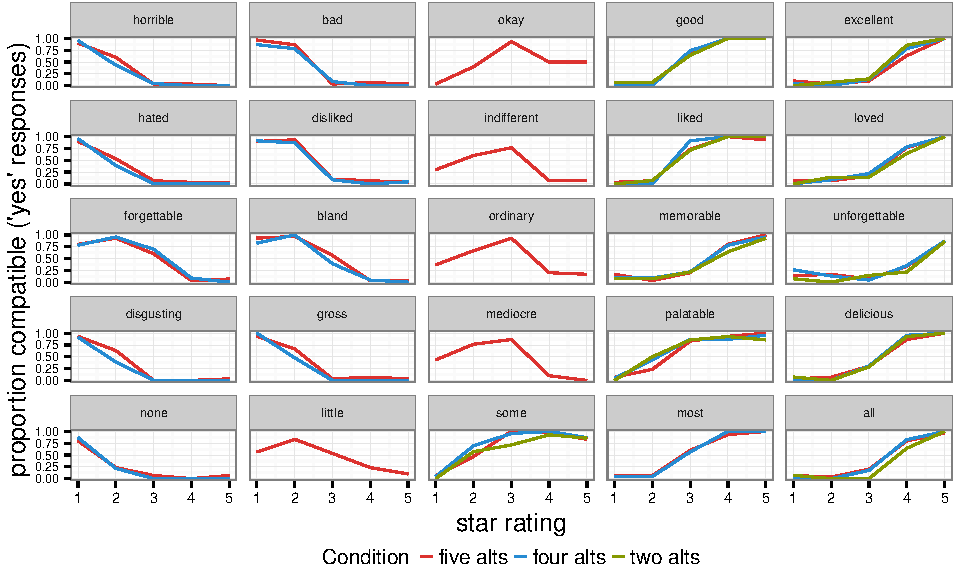
\includegraphics{figs/exp1Plots-1} 

}

\caption[The left panel plots literal semantic distributions for the scalar pair 'liked/loved']{The left panel plots literal semantic distributions for the scalar pair 'liked/loved'. The y-axis is the percentage of 'yes' responses for a scalar term that is compatibible with the number of stars on the x-axis (ie 100\% of respondents beleived that 'liked' was compatible with both 4 and 5 stars). Erro bars are 95\% confidence intervals. The right panel plots pragmatic judgments for the scalar pair 'liked/loved'. The y-axis is the proportion of selection of the star-rating on the x-axis (ie over 80\% of judgments when prompted with 'loved' were 5-stars).}\label{fig:exp1Plots}
\end{figure*}
\end{CodeChunk}

\section{Experiment 2: What are the
alternatives?}\label{experiment-2-what-are-the-alternatives}

In Experiment 1 we obtained literal semantic compatibility and pragmatic
judgments for five pairs of scalar terms. We would like to extend the
scale descriptions for each of these pairs to include other plausible
alternatives. We chose to take an empirical approach rather than assign
alternatives arbitrarily. We adopted a modified cloze task, inspired by
Experiment 2 in van Tiel (2014) and asked participants to generate
alternatives for us.

\subsection{Methods}\label{methods-1}

\subsubsection{Participants}\label{participants-1}

Using Amazon's Mechanical Turk, 30 workers were paid \$0.20 to
participate. All participants were native English speakers and naive to
the purpose of the experiment.

\subsubsection{Design and procedure}\label{design-and-procedure-1}

Participants were presented a target scalar term from our original
entailment set embedded in a sentence such as, ``In a recent restaurant
review someone said they thought they the food was \_\_\_\_" with a
target scalar presented in the ``\_\_\_\_." Participants were then asked
to generate plausible alternatives by responding to the question, ``If
they'd felt differently about the food, what other words could they have
used instead of \_\_\_\_\_?'' and asked to generate three unique
alternatives.

\subsection{Results and Discussion}\label{results-and-discussion-1}

Figure 3 plots the combined counts of alternatives generated for the
scalar items ``liked'' and ``loved.'' Alternative distributions for the
other scalar pairs (e.g.. ``good/excellent'',
``memorable/unforgettable'') were similarly long-tailed, however the
size and content of the alternate sets were diverse. (SOMETHING MORE
MORE FORMAL HERE???)

\begin{CodeChunk}
\begin{figure*}[t]

{\centering 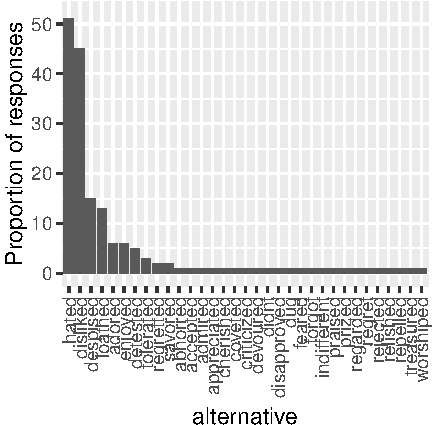
\includegraphics{figs/exp2_altsPlot_likedLoved-1} 

}

\caption[Caption goes here]{Caption goes here}\label{fig:exp2_altsPlot_likedLoved}
\end{figure*}
\end{CodeChunk}

\section{Experiment 3a,b: Incorporating top
alternatives}\label{experiment-3ab-incorporating-top-alternatives}

In Experiment 1a,b we measured literal semantics and pragmatic judgments
for Entailment scales. In Experiment 2, we asked participants to
generate plausible alternatives to these items. In Experiments 3a,b we
use the same experimental design for both literal semantics and
pragmatic judgment tasks, however we now expand the set of scalar items
to include the original Entailment pairs from Experiments 1a,b with the
top two alternatives generated for each scalar family by participants in
Experiment 2. The orange colored items in table 1 denote additional
scalar items added in Experiments 3a,b.

\subsection{Participants}\label{participants-2}

Participants for both studies were recruited on Amazon Mechanical Turk
and paid \$0.20 for their participation. Thirty participants were
recruited for Experiment 3a (Literal Listener task). Data for six
participants was thrown out after participants either failed to pass two
training trials or were not native English speakers, leaving a total
sample of 24 participants.

Fifty participants were recruited for Experiment 3b (Pragmatic Listener
task). Data for five participants was thrown out after participants
either failed to pass two training trials or were not native English
speakers, leaving a total sample of 45 participants.

\subsection{Procedure}\label{procedure}

The procedure of Experiments 3a,b follow the same form as Experiments
1a,b with the expanded set of target scalar items.

\subsection{Results and Discussion}\label{results-and-discussion-2}

Run glmer() here:

To test whether literal listener compatibility judgments differed
between Experiment 1a and 3a we ran a mixed effects model, regressing
responses to the binary compatibility measure on scale, degree, and
Experiment with random effects by subject. Results indicate (\ldots{})

Run elmer() here:

To test whether pragmatic judgments differed between Experiments 1b and
3b we ran a mixed effects model, regressing star-rating selections on
scale, scalar item and Experiment with random effects by subject.
Results indicate.

While conducting our analysis we realized that our literal semantic
distributions for each scalar family were roughly split between two
negative valenced items and two positively valenced items while neutral
alternatives appeared to be excluded. (This pattern was true of all the
scalar families, except for ``some ~all'' in which the top two
alternatives were positive valenced ``most'' and negative valenced
``none''.) In Experiment 4, we explore the addition of a neutrally
valenced scalar alternative for each scalar family.

\section{Experiment 4: Full scales - adding a neutral
alternative}\label{experiment-4-full-scales---adding-a-neutral-alternative}

In Experiment 4, we continue to extend the alternative sets, each by one
additional scalar item. While we simply took the top two alternatives
generated in Experiment 2 for the additional alternatives in Experiments
3a,b, in this case we chose a subjectively ``neutral'' valenced scalar
item from among the alternatives generated in Experiment 2. The idea was
to simulate a ``full'' set of alternatives, with negative, neutral and
positive valenced items for each scalar family. The purple colored items
in Table 1 denote additional scalar items added in Experiments 4.

\subsection{Participants}\label{participants-3}

Thirty participants were recruited on Amazon Mechanical Turk and paid
\$0.20 for their participation. There were no data exclusions due to
training failures or native language requirements, leaving a total
sample of thirty participants, all native English speakers, naive to the
purpose of the experiment.

\subsection{Procedure}\label{procedure-1}

The procedure of Experiment 4 follow the same form as Experiments 1a and
3a with the addition of a neutrally valence scalar item.

\subsection{Results and Discussion}\label{results-and-discussion-3}

Distributions for neutrally valenced scalar did appear fairly Gaussian,
occupying a literal semantic previously unoccupied by the other
alternatives.

Run glmer() here:

To test whether literal listener compatibility judgments differed
between Experiment 1a and 3a we ran a mixed effects model, regressing
responses to the binary compatibility measure on scale, degree, and
Experiment with random effects by subject. Results indicate (\ldots{})

Run elmer() here:

To test whether pragmatic judgments differed between Experiments 1b and
3b we ran a mixed effects model, regressing star-rating selections on
scale, scalar item and Experiment with random effects by subject.
Results indicate.

\section{Model Runs}\label{model-runs}

Using literal semantic data from Experiments 1a, 3a and 4 we conducted
three simulations with our model. Each simulation used the specific
literal semantic data to specify the scale representation available to
our model. The ``entailment'' model used only the original pair of
scalar items pulled from van Tiel (2014). These data were measured in
Experiment 1a. The ``Top two'' model extended the original set of
alternatives with the top two alternatives generated in Experiment 2.
These data were measured in Experiment 3a. The ``Full'' model included
the full set of alternatives, including a neutral valenced alternative.
These data were measured in Experiment 4.

\begin{CodeChunk}
\begin{figure*}[t]

{\centering 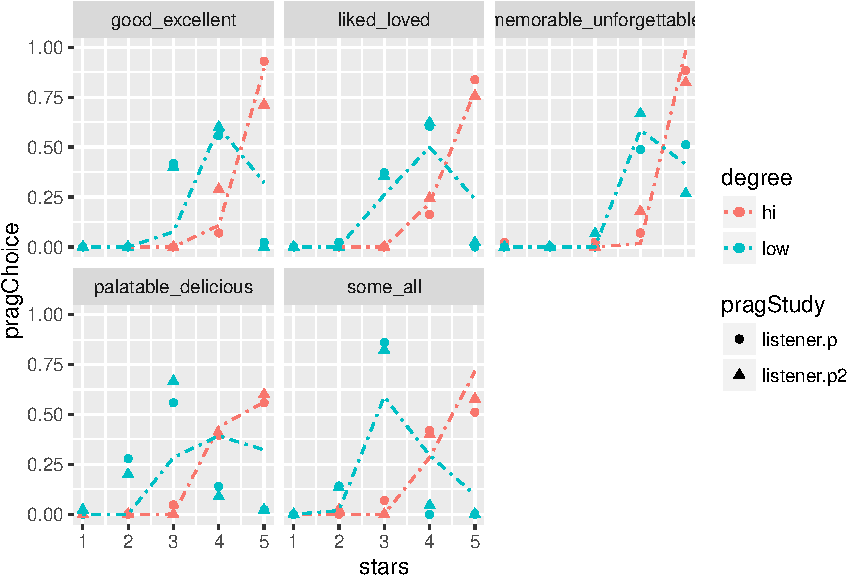
\includegraphics{figs/performancePlots-1} 

}

\caption[The left panel shows improved model fit as scale representations are enriched with more scalar items]{The left panel shows improved model fit as scale representations are enriched with more scalar items. Correlations are coputed using pragmatic judgment data from Experiments 1b and 3b. The right panel plots model predictions using full symmetric scales versus human judgments from Experiment 3b.}\label{fig:performancePlots}
\end{figure*}
\end{CodeChunk}

\section{General Discussion}\label{general-discussion}

By varying the type of scale representations available to our Bayesian
model we investigated the effects of alternatives on scalar implicature.
Model fit with human judgement was significantly improved by the
inclusion of alternatives beyond the typical ``strong'' and ``weak''
scalar items. In fact, we found that both neutral and negative valence
scalar items contribute to human-like implicature generation within our
framework.

\textbackslash{}begin\{CodeChunk\}
\textbackslash{}begin\{figure\}{[}h{]}

\{\centering 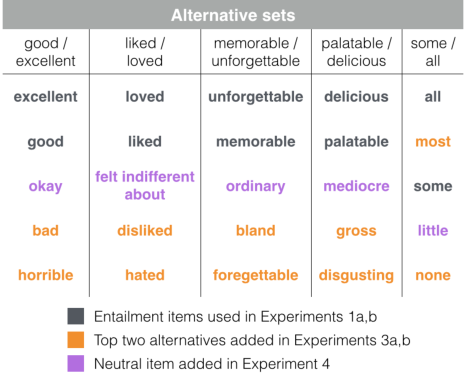
\includegraphics{figs/allScalesTable-1}

\}

\textbackslash{}caption{[}This table shows the stimuli used in
Experiments 1a,b, 3a,b and 4{]}\{This table shows the stimuli used in
Experiments 1a,b, 3a,b and 4. Colors denote the additions made in each
experiment. For example, in Experiment 1a we measured literal semantics
for `liked/loved'. In Experiment 3a,b we extended this group to
`textit\{hated/disliked/liked/loved'. In Experiment 4 we extended this
grou to `hated/disliked/felt indifferent
about/liked/loved'.\}\label{fig:allScalesTable}
\textbackslash{}end\{figure\} \textbackslash{}end\{CodeChunk\}

\section{Acknowledgements}\label{acknowledgements}

Thanks to NSF BCS XYZ. Thanks to Michael Franke, Judith Degen, and Noah
Goodman.

\section{References}\label{references}

\setlength{\parindent}{-0.1in} \setlength{\leftskip}{0.125in} \noindent

Ignore below this

use a food review paradigm in which `meaning' for a given scalar item
was quantified as a distribution over star-ratings. Quantifying both
literal semantic content and pragmatic judgments as distributions over
stars provides an important interface to our model, especially for
scalar items with ambiguous literal semantics (e.g.~items such as
``liked/loved'' or ``memorable/unforgettable''). In addition to
quantifying literal semantics and pragmatic judgments in Experiments
1a,b and Experiments 3a,b, Experiment 2 used a modified cloze task,
based on van Tiel (2013, Experiment 2???), to generate a set of
plausible alternatives to the scalar items used in Experiments 1a,b. We
extend the set of alternatives measured in Experiments 3a,b and 4 using
data from Experiment 2. Additionally, by looking at the relative
frequencies of alternatives generated in Experiment 2 we were able to
compute a saliency measure for each alternative. Using the literal
semantic data from Experiments 1a, 3a and 4, we modeled pragmatic
enrichment using RSA and compared model predictions to human judgments
obtained in Experiments 1b and 3b. Model performance was significantly
improved with the incorporation of alternatives. This result suggests
that more ``fully specified" scale representations may be active for
human participants while making pragmatic judgments for scalar items.

\end{document}
